%% REPLACE sXXXXXXX with your student number
\def\studentNumber{s2177402}


%% START of YOUR ANSWERS
%% Add answers to the questions below, by replacing the text inside the brackets {} for \youranswer{ "Text to be replaced with your answer." }. 
%
% Do not delete the commands for adding figures and tables. Instead fill in the missing values with your experiment results, and replace the images with your own respective figures.
%
% You can generally delete the placeholder text, such as for example the text "Question Figure 2 - Replace the images ..." 
%
% There are 19 TEXT QUESTIONS (a few of the short first ones have their answers added to both the Introduction and the Abstract). Replace the text inside the brackets of the command \youranswer with your answer to the question.
%
% There are also 3 "questions" to replace some placeholder FIGURES with your own, and 3 "questions" asking you to fill in the missing entries in the TABLES provided. 
%
% NOTE! that questions are ordered by the order of appearance of their answers in the text, and not by the order you should tackle them. Specifically, you cannot answer Questions 2, 3, and 4 before concluding all of the relevant experiments and analysis. Similarly, you should fill in the TABLES and FIGURES before discussing the results presented there. 
%
% NOTE! If for some reason you do not manage to produce results for some FIGURES and TABLES, then you can get partial marks by discussing your expectations of the results in the relevant TEXT QUESTIONS (for example Question 8 makes use of Table 1 and Figure 2).
%
% Please refer to the coursework specification for more details.


%% - - - - - - - - - - - - TEXT QUESTIONS - - - - - - - - - - - - 

%% Question 1:
\newcommand{\questionOne} {
\youranswer{Overfitting is making prediction too strict in order to produce consistent predictions in a particular data set, so that it can not predict data well on test sets or other data sets.}
}

%% Question 2:
\newcommand{\questionTwo} {
\youranswer{With the increase of the width and depth of the architecture, the generalization gap increases and the overfitting becomes more obvious.}
}

%% Question 3:
\newcommand{\questionThree} {
\youranswer{both Dropout and L1/L2 penalty can alleviate overfitting, but appropriate hyperparameters need to be selected (excessive hyperparameters can affect the model fitting, resulting in poor validation accuracy).
The optimal hyperparameters of the two methods do not mean that their combination will bring the best results.}
}

%% Question 4:
\newcommand{\questionFour} {
\youranswer{Both methods and their combination can alleviate overfitting and improve the performance of the model (provided that appropriate hyperparameters are selected). Future experiments will consider adding Maxout as a new activation function.}
}

%% Question 5:
\newcommand{\questionFive} {
\youranswer{Overfitting is a phenomenon that model has too good results on the training set and not so good results on the test set. For example with the progress of learning epochs, the accuracy rate decreases or does not increase like that on training set and generalization gap increases sharply especially on test set.}
}

%% Question 6:
\newcommand{\questionSix} {
\youranswer{Overfitting occurs for a number of reasons. First, the modeling sample set is incorrectly selected. For example, the number of sample sets is too small, leading to the sample data is not enough to represent the predetermined classification. Second, the noise contained in the sample set is too large, leading to the machine to regard part of the noise as valid data and thus interfere with the classification. Thirdly, the model has too many parameters and too much complexity (too much width and depth). In general, when the error rate of the model in the validation set is not significantly reduced or even increases with the number of learning rounds, or the generalization gap is extremely large, we can think that overfitting has occurred. From a practical point of view, the most important point is the classification accuracy, and when the classification accuracy on the test set no longer increases with that of the training set, it can be considered that there is an overfitting.}
}

%% Question 7:
\newcommand{\questionSeven} {
\youranswer{These two figures reflect the performance of classification accuracy and cross entropy errors in training set and verification set. As you can see from these two graphs, both of them are steadily rising or falling in the training set. However, in the validation set, after the vertex of the image curve (the point with slope 0), the two develop in reverse. The cross entropy error shows an upward trend around the 15th epoch, which can be considered as a sign of overfitting. But from a practical point of view, what we really care about is improving the classification accuracy on the validation data, so we think that the vertex of the classification accuracy curve on the validation set is the point where overfitting begins to dominate learning.}
}

%% Question 8:
\newcommand{\questionEight} {
\youranswer{From Table 1 and Figure 2, we can see that with the increase of model width, the accuracy rate of prediction increases continuously in the training set. But the results on the validation set were roughly the same (around 0.8). As the width of the model increases, the cross entropy error decreases in the training set, but the generalization gap increases (from 0.148 to 0.811).At the same time, around the 20th epoch, the models with width 64 and 128 appeared overfitting (the accuracy on validation set stops increasing and the errors in the validation set increased rather than decreased).}
}

%% Question 9:
\newcommand{\questionNine} {
\youranswer{From the images and data, it can be seen that the model with width 32 is underfitting (the result on the verification set is much lower than the result on the training set), the model with width 64 and 128 is overfitting, and the model with width 128 is overfitting more seriously.
To some extent, this confirms the previous explanation of the cause of overfitting and the possibility of overfitting is higher when the model complexity is too high.}
}

%% Question 10:
\newcommand{\questionTen} {
\youranswer{On the training set, the classification accuracy becomes higher and the errors become lower as the depth of the model increases. However, in the validation set, the classification accuracy of the three models is roughly the same (only slightly improved with the increase of depth), and the error and generalization gaps become larger with the increase of depth.}
}

%% Question 11:
\newcommand{\questionEleven} {
\youranswer{The effects of different depths on the results are consistent. As the depth of the model increases, the classification accuracy becomes higher in both sets, even if it is very small in the validation set. On the validation set, error and generalization gaps become larger with increasing depth.
This is consistent with the previous description of over-complex models leading to overfitting. As can be seen from the generalization gap, the overfitting of the model becomes more serious with the increase of depth.}
}

%% Question 12:
\newcommand{\questionTwelve} {
\youranswer{With the increase of model complexity (width and depth), the performance of the model increases little, but the degree of overfitting increases significantly.}
}

%% Question 13:
\newcommand{\questionThirteen} {
\youranswer{In machine learning, the loss function is usually followed by an extra term. There are two common extra terms, L1-norm and L2-norm.
These two can be viewed as the penalty terms of the loss function.

L1-norm refers to the sum of the absolute values of each element in the weight vector W, usually expressed as \begin{equation}
\| \boldsymbol{v} \|_1 = \sum_{d=1}^D \left| v_d \right|,
\end{equation}
To weigh the penalty term, add a positive scalar coefficient, $\beta_i$.\begin{equation}
  C^{(i)}_{\textrm{L1}} = 
  \beta_i \left\| \boldsymbol{p}^{(i)} \right\|_1 = 
  \beta_i  \sum_{d=1}^D \left| p^{(i)}_d \right|.
\end{equation}
The gradient of the parameter vector is \begin{equation}
  \frac{\partial C^{(i)}_{\textrm{L1}}}{\partial p^{(i)}_d} = \beta_i \, \textrm{sgn}\left( p^{(i)}_d \right)
\end{equation}


L2-norm refers to the sum square root of the squares of each element in the weight vector W, and is defined as.\begin{equation}
\| \boldsymbol{v} \|_2 = \left[ \sum_{d=1}^D \left( v_d^2 \right) \right]^{\frac{1}{2}}.
\end{equation}
Similarly, to weigh the penalty term, add a positive scalar coefficient, $\beta_i$.\begin{equation}
  C^{(i)}_{\textrm{L2}} = 
  \frac{1}{2} \beta_i \left\| \boldsymbol{p}^{(i)} \right\|_2^2 =
  \frac{1}{2} \beta_i \sum_{d=1}^D \left[ \left( p^{(i)}_d \right)^2 \right].
\end{equation}
And notice that $\frac{1}{2}$ isn't necessary here, we're just trying to figure out the gradient later, so that $\frac{1}{2}$ and 2 can multiply and cancel out to 1.\begin{equation}
  \frac{\partial C^{(i)}_{\textrm{L2}}}{\partial p^{(i)}_d} = \beta_i p^{(i)}_d
\end{equation}

L1 and L2 penalties are very easy to implement. It can be implemented in an AffineLayer, adding the gradient of the penalty term to the existing gradient and returning the penalty term of the layer dependent parameter. The gradient of the penalty term and the penalty term themselves can be calculated by the function according to the formula. The function parameter which can be adjusted freely is the coefficient before the penalty term.
}
}

%% Question 14:
\newcommand{\questionFourteen} {
\youranswer{During the fitting process, it is generally preferred to keep the weights as small as possible and construct a model with relatively small parameters. Because it is generally considered that the model with smaller parameter value is relatively simple and can avoid the over-fitting phenomenon to a certain extent. In the gradient descent algorithm, L2-norm iteratively multiplizes a factor less than 1 to make the result progressively smaller, resulting in a smaller parameter (called weight decay). Unlike L2-norm, L1-norm can generate a sparse weight matrix for feature selection. Many elements in the sparse matrix are 0, and only a few elements are non-zero, that is, the coefficients of weights. The end result is that L1-norm tends to focus its weight on high-importance connections, while others have a weight of 0. This also reduces the complexity of the model, so it can prevent overfitting to a certain extent.}
}

%% Question 15:
\newcommand{\questionFifteen} {
\youranswer{As can be seen from Table 3 and Figure 4a/b, for dropout, the smaller the selected parameters are, the smaller the generalization gap is (the probability of neuron inactivation at each layer increases, thus reducing the complexity of the model), which alleviates overfitting to some extent.
When the probability is selected as 0.7, the validation accuracy is lower than the baseline, which indicates that this probability will make the model too simple to fit well.

For L1 and L2 penalty, the larger the parameter selection is, the smaller the generalization gaps are, which can alleviate the overfitting. However, when 1e-1 is selected, the validation accuracy of the model is extremely low, indicating that the excessive penalty value will interfere with the correct fitting of the model.

Therefore, for the combined experiment, parameters with validation accuracy higher than the baseline were selected in order to obtain a better fitting effect. The six combinations are shown in Table 3.

As can be seen from Table 3 and Figure 4c, the combination of 0.9 and L2 1e-4 has the highest validation accuracy; the test accuracy of 0.95 and L2 1e-4 is very close, but it has the highest generalization gap. Therefore, 0.9 and L2 1e-4 are the optimal combination.
Surprisingly, the parameters that achieved the best results in the previous Dropout and L1/L2 penalty, 0.95 and L2 1e-3, did not achieve the optimal validation accuracy, which means that the combination of multiple methods still needs to be tested in practice, and it is not possible to determine the optimal combination based on the results of a single method.}
}

%% Question 16:
\newcommand{\questionSixteen} {
\youranswer{Maxout was proposed to optimize the accuracy of dropout and dropout fitting model averaging processes.
Relu has a gradient attenuation problem at the lower level, and when the gradient does not change with the dropout mask, the dropout is simplified to SGD.
The linear and maximization operations in Maxout allow the approximations of model averaging to be precise.}
}

%% Question 17:
\newcommand{\questionSeventeen} {
\youranswer{Maxout is essentially an activation function. So it can be used with dropout. Maxout also has the advantages of Relu without its disadvantages (neuronal death). When using dropout, the dropout operation precedes the matrix multiplication, not the maxout operation.}
}

%% Question 18:
\newcommand{\questionEighteen} {
\youranswer{The experiment evaluated the Maxout model on four benchmark datasets (MNIST,CIFAR-10,CIFAR-100,SVHN),through testing on these data sets, Maxout obtained very advanced results. The researchers then built a rectifier of the same size as Maxout for a control experiment, and the results were still good.To demonstrate that Maxout works better with Dropout, the researchers compared it with Tanh and Dropout. Maxout turned out to have better performance. The reasoning process covers a wide range of data sets and uses controlled trials, so the conclusion is convincing.}
}

%% Question 19:
\newcommand{\questionNineteen} {
\youranswer{By training multiple models of different complexity (width and depth), we found that the higher the complexity of the model, the higher the degree of overfitting. But too simple models will lead to underfitting. So choosing the right model size is very important. We then tested two different methods for preventing overfitting (Dropout and L1/L2 penalty) and selected the hyperparameters with better results for the combination experiment. The results show that these two methods can alleviate the overfitting and improve the performance of the model(Validation Accuracy). But the combination experiment tells us that the hyperparameter combination with the best result is not necessarily optimal. Maxout, a special activation function, is introduced at the end of the article. In future experiments Maxout will be considered to replace Relu, and their combination with the Dropout and L1/L2 PENALTY will be evaluated}
}


%% - - - - - - - - - - - - FIGURES - - - - - - - - - - - - 

%% Question Figure 2:
\newcommand{\questionFigureTwo} {
\youranswer{Question Figure 2 - Replace the images in Figure 2 with figures depicting the accuracy and error, training and validation curves for your experiments varying the number of hidden units.
%
\begin{figure}[t]
    \centering
    \begin{subfigure}{\linewidth}
        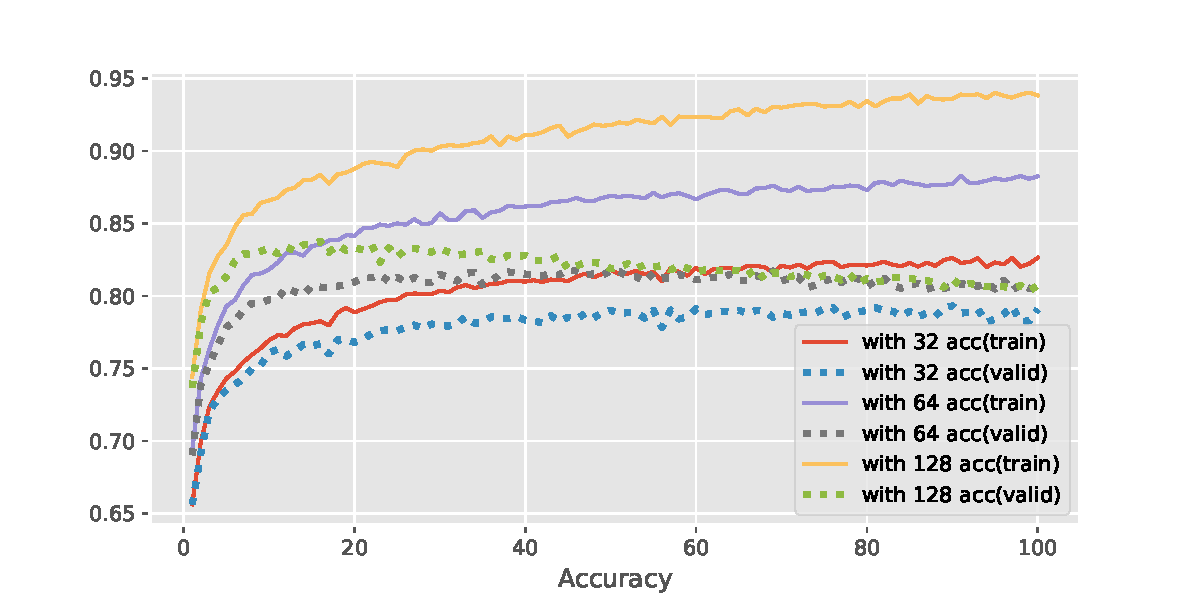
\includegraphics[width=\linewidth]{figures/empty_acc_curve_width_1.pdf}
        \caption{accuracy by epoch}
        \label{fig:width_acccurves}
    \end{subfigure} 
    \begin{subfigure}{\linewidth}
        \centering
        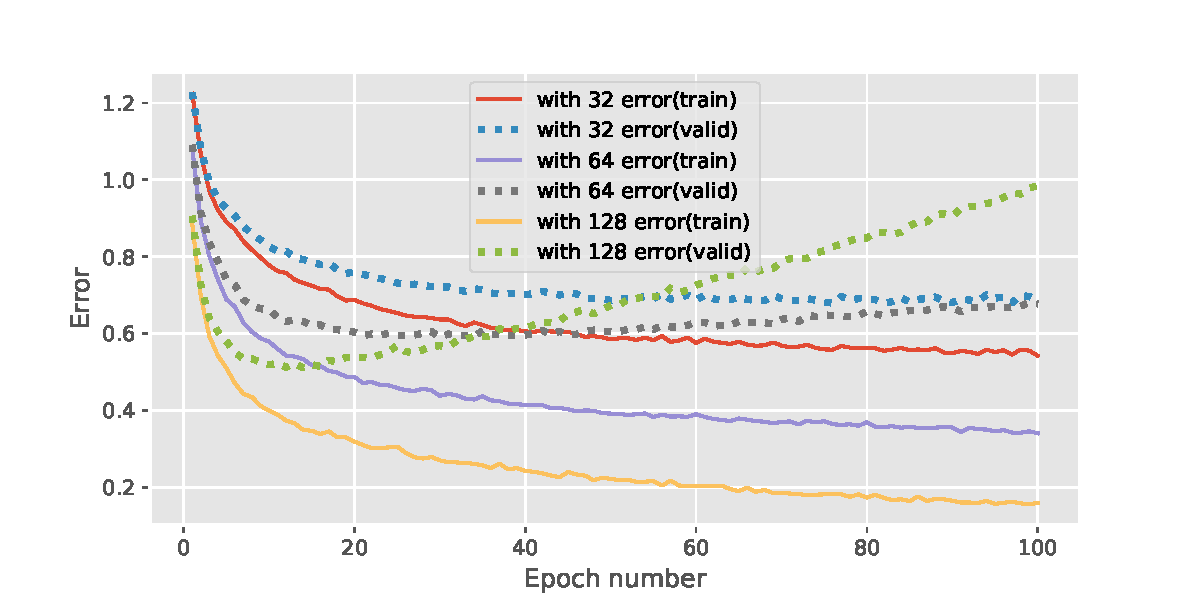
\includegraphics[width=\linewidth]{figures/empty_error_curve_width_1.pdf}
        \caption{error by epoch}
        \label{fig:width_errorcurves}
    \end{subfigure} 
    \caption{Training and validation curves in terms of classification accuracy (a) and cross-entropy error (b) on the EMNIST dataset for different network widths.}
    \label{fig:width}
\end{figure} 
}
}

%% Question Figure 3:
\newcommand{\questionFigureThree} {
\youranswer{Question Figure 3 - Replace these images with figures depicting the accuracy and error, training and validation curves for your experiments varying the number of hidden layers.
%
\begin{figure}[t]
    \centering
    \begin{subfigure}{\linewidth}
        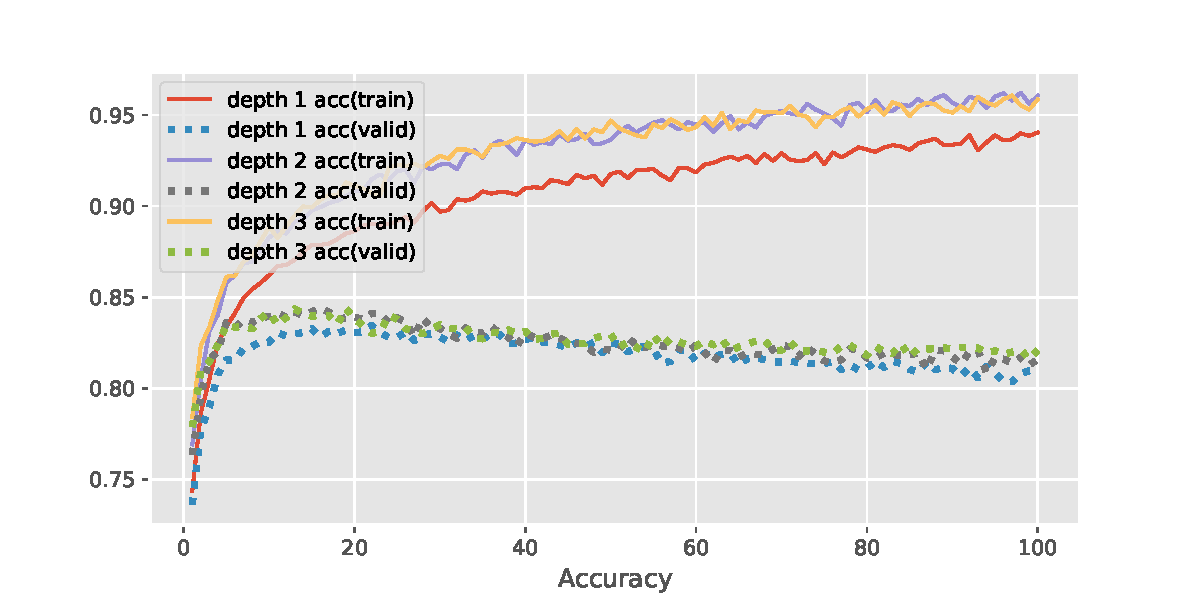
\includegraphics[width=\linewidth]{figures/empty_acc_curve_depth_1.pdf}
        \caption{accuracy by epoch}
        \label{fig:depth_acccurves}
    \end{subfigure} 
    \begin{subfigure}{\linewidth}
        \centering
        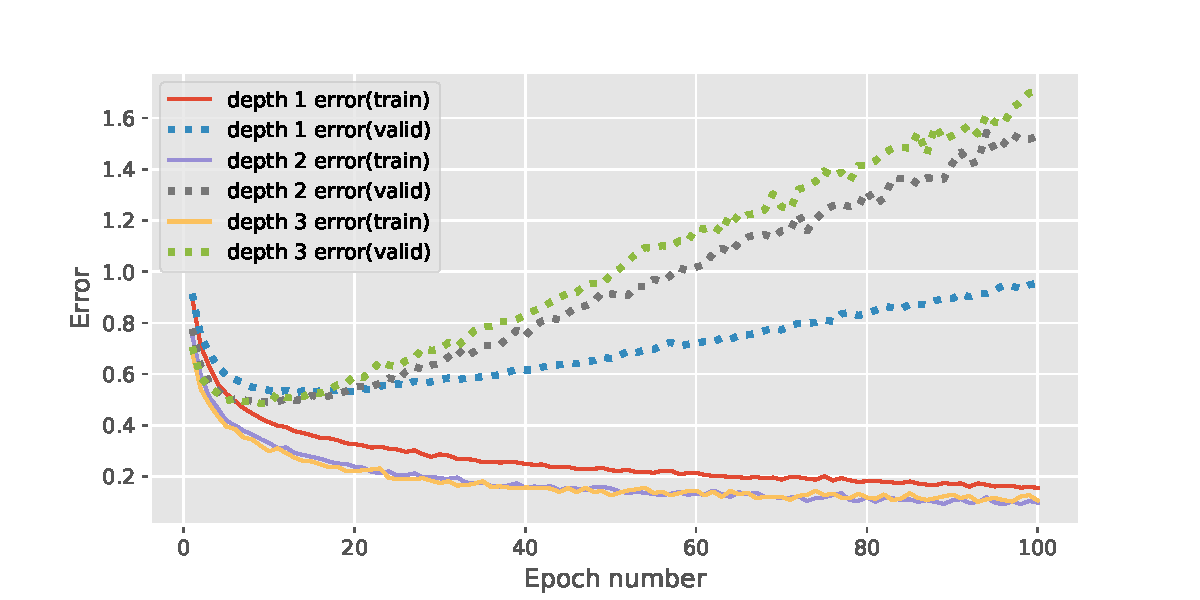
\includegraphics[width=\linewidth]{figures/empty_error_curve_depth_1.pdf}
        \caption{error by epoch}
        \label{fig:depth_errorcurves}
    \end{subfigure} 
    \caption{Training and validation curves in terms of classification accuracy (a) and cross-entropy error (b) on the EMNIST dataset for different network depths.}
    \label{fig:depth}
\end{figure} 
}
}

%% Question Figure 4:
\newcommand{\questionFigureFour} {
\youranswer{Question Figure 4 - Replace these images with figures depicting the Validation Accuracy and Generalisation Gap for each of your experiments varying the Dropout inclusion rate, L1/L2 weight penalty, and for the 8 combined experiments (you will have to find a way to best display this information in one subfigure).
%
\begin{figure*}[t]
    \centering
    \begin{subfigure}{.3\linewidth}
        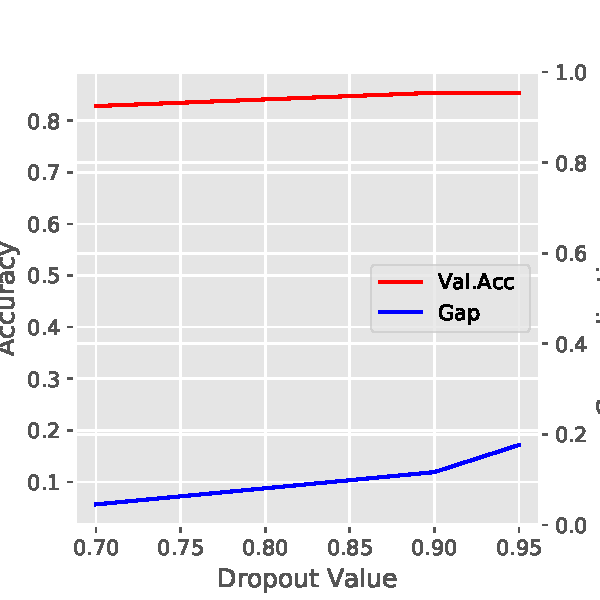
\includegraphics[width=\linewidth]{figures/empty_dropout_plot_1.pdf}
        \caption{Metrics by inclusion rate}
        \label{fig:dropoutrates}
    \end{subfigure} 
    \begin{subfigure}{.3\linewidth}
        \centering
        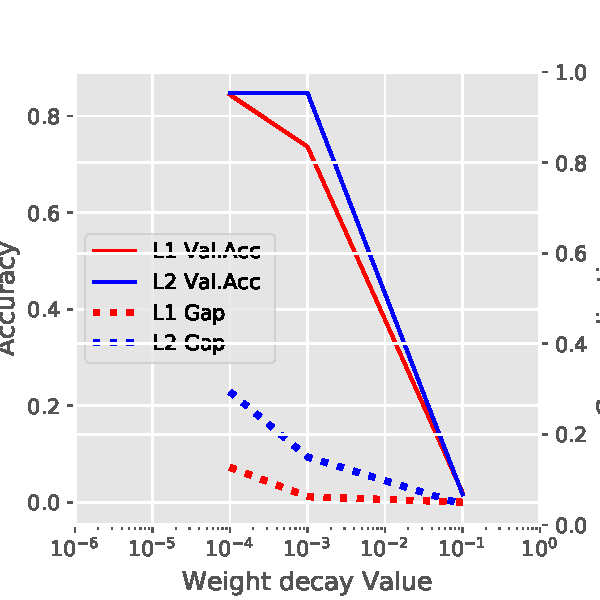
\includegraphics[width=\linewidth]{figures/empty_wd_plot_1.pdf}
        \caption{Metrics by weight penalty}
        \label{fig:weightrates}
    \end{subfigure} 
    \begin{subfigure}{.3\linewidth}
        \centering
        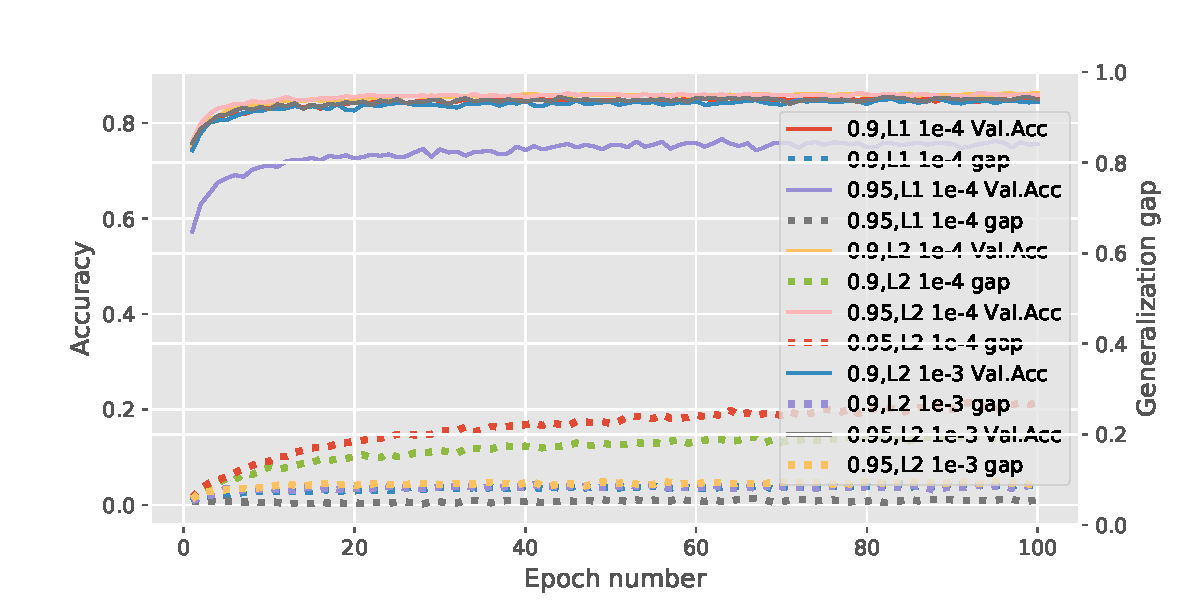
\includegraphics[width=.85\linewidth]{figures/extra.pdf}
        \caption{Extra experiments}
        \label{fig:extra}
    \end{subfigure} 
    \caption{Hyperparameter search for every method and combinations}
    \label{fig:hp_search}
\end{figure*}
}
}

%% - - - - - - - - - - - - TABLES - - - - - - - - - - - - 

%% Question Table 1:
\newcommand{\questionTableOne} {
\youranswer{
Question Table 1 - Fill in Table 1 with the results from your experiments varying the number of hidden units.
%
\begin{table}[t]
    \centering
    \begin{tabular}{c|cc}
    \toprule
        \# hidden units & val. acc. & generalization gap \\
    \midrule
         32            & 0.788           & 0.148                   \\
         64            & 0.805           & 0.344                   \\
         128           & 0.807           & 0.811                   \\ 
    \bottomrule
    \end{tabular}
    \caption{Validation accuracy (\%) and generalization gap (in terms of cross-entropy error) for varying network widths on the EMNIST dataset.}
    \label{tab:width_exp}
\end{table}
}
}

%% Question Table 2:
\newcommand{\questionTableTwo} {
\youranswer{
Question Table 2 - Fill in Table 2 with the results from your experiments varying the number of hidden layers.
%
\begin{table}[t]
    \centering
    \begin{tabular}{c|cc}
    \toprule
        \# hidden layers & val. acc. & generalization gap \\
    \midrule
         1               & 0.809           & 0.800                   \\
         2               & 0.816           & 1.432                   \\
         3               & 0.821           & 1.594                   \\ 
    \bottomrule
    \end{tabular}
    \caption{Validation accuracy (\%) and generalization gap (in terms of cross-entropy error) for varying network depths on the EMNIST dataset.}
    \label{tab:depth_exps}
\end{table}
}
}

%% Question Table 3:
\newcommand{\questionTableThree} {
\youranswer{
Question Table 3 - Fill in Table 3 with the results from your experiments varying the hyperparameter values for each of L1 regularisation, L2 regularisation, and Dropout (use the values shown on the table) as well as the results for your experiments combining L1/L2 and Dropout (you will have to pick what combinations of hyperparameter values to test for the combined experiments; each of the combined experiments will need to use Dropout and either L1 or L2 regularisation; run an experiment for each of 8 different combinations). Use \textit{italics} to print the best result per criterion for each set of experiments, and \textbf{bold} for the overall best result per criterion.
%
\begin{table*}[t]
    \centering
    \begin{tabular}{c|c|cc}
    \toprule
        Model    &  Hyperparameter value(s) & Validation accuracy & Generalization gap \\
    \midrule
    \midrule
        Baseline &  -                    &               0.836 &                 0.290 \\
    \midrule
        \multirow{3}*{Dropout}
                 & 0.7                   &  \textit{0.832}                   & \textit{0.060}                  \\
                 & 0.9                   &  \textit{0.857}                   & \textit{0.129}                  \\   
                 & 0.95                  &  \textbf{0.860}                   & \textbf{0.168}                  \\
    \midrule
        \multirow{3}*{L1 penalty}
                 & 1e-4                   & \textbf{0.847}                    & \textbf{0.077}                  \\
                 & 1e-3                   & \textit{0.752}                    & \textit{0.010}                  \\
                 & 1e-1                   & \textit{0.046}                    & \textit{0.0004}                  \\
    \midrule
        \multirow{3}*{L2 penalty}  
                 & 1e-4                   & \textit{0.845}                    & \textit{0.236}                  \\
                 & 1e-3                   & \textbf{0.852}                    & \textbf{0.096}                  \\
                 & 1e-1                   & \textit{0.019}                    & \textit{-0.004}                  \\
    \midrule
        \multirow{6}*{Combined}  
                 & for example 0.95, L1 1e-6  &                     &                   \\
                 & 0.9,L1 1e-4                   & \textit{0.856}                    & \textit{0.038}                  \\
                 & 0.95,L1 1e-4                   & \textit{0.763}                    & \textit{0.017}                  \\
                 & 0.9,L2 1e-4                   & \textbf{0.863}                    & \textbf{0.14}                  \\
                 & 0.95,L2 1e-4                   & \textit{0.863}                    & \textit{0.206}                  \\
                 & 0.9,L2 1e-3                   & \textit{0.851}                    & \textit{0.037}                  \\
			 & 0.95,L2 1e-3                   & \textit{0.855}                    & \textit{0.046}                  \\
    \bottomrule
    \end{tabular}
    \caption{Results of all hyperparameter search experiments. \emph{italics} indicate the best results per series and \textbf{bold} indicate the best overall}
    \label{tab:hp_search}
\end{table*}
}
}

%% END of YOUR ANSWERS